% ECO372H5F -- Problem Set 1 -- policy memo template
% Put your prose in the body. The results TABLE is pulled straight
% from your Stata output -- you never retype a number.
%
% Compile in Overleaf, or locally with pdflatex. The \input line
% below reads output/results.tex, which 03_analysis.do writes.
\documentclass[11pt]{article}
\usepackage[margin=1in]{geometry}
\usepackage{booktabs}
\usepackage{graphicx}
\begin{document}

\begin{flushleft}
\textbf{To:} Hon. Trevor Jones, Ministry of Labour \\
\textbf{From:} Raunak Boparai \\
\textbf{Re:} Does the job-training program raise earnings? \\
\hrulefill
\end{flushleft}

% --- your memo goes here (about one page, no equations, no jargon) ---
The randomized experiment gives the best evidence that the job-training program increased earnings. I would use the estimate in column (1) as the main estimate of the program's effect. The estimate in column (2), after adding controls, is fairly similar. This makes sense because people were randomly assigned to the training and control groups, so the comparison does not depend on the types of people who chose to receive training. Based on these results, I would not recommend scaling back the program because of the smaller observational estimate.

\bigskip
The observational results are less reliable. The trainees are compared with the people from the PSID who were already very different before the training took place. One clear example is their earnings in 1975, when the training group had much lower earnings than the PSID group. The observational estimate also changes dramatically once controls are added, showing how much the result depends on differences between the two groups. Adding controls for age, education, race, marital status, and earlier earnings can account for differences we can measure, but it does not make the groups the same as if they had been randomly assigned. There may still be other differences between them that are not included in the data. For this reason, I would not treat the estimate in column (4) as the causal effect of the program.

\bigskip
Overall, I am fairly confident that the program increased 1978 earnings for the people represented in this experiment, although I am less certain about the exact size of the increase. The experimental result is more convincing because the treatment and control groups were created through a random assignment. I would use this result when judging the benefits of the program and then compare those benefits with the cost of running it before deciding whether the program should be expanded or reduced. I would be less confident in this conclusion if there were problems with the way the random assignment was carried out or if another well-run randomized study found little or no increase in earnings.

\bigskip
% --- results pulled directly from Stata (do not retype numbers) ---
{
\def\sym#1{\ifmmode^{#1}\else\(^{#1}\)\fi}
\begin{tabular}{l*{4}{c}}
\hline\hline
            &\multicolumn{1}{c}{(1)}&\multicolumn{1}{c}{(2)}&\multicolumn{1}{c}{(3)}&\multicolumn{1}{c}{(4)}\\
            &\multicolumn{1}{c}{re78}&\multicolumn{1}{c}{re78}&\multicolumn{1}{c}{re78}&\multicolumn{1}{c}{re78}\\
\hline
treat       &      1794.3\sym{**} &      1675.9\sym{**} &    -15204.8\sym{***}&       795.0         \\
            &     (632.9)         &     (639.3)         &    (1154.6)         &     (915.8)         \\
\hline
\(N\)       &         445         &         445         &        2675         &        2675         \\
\hline\hline
\multicolumn{5}{l}{\footnotesize Standard errors in parentheses}\\
\multicolumn{5}{l}{\footnotesize \sym{*} \(p<0.05\), \sym{**} \(p<0.01\), \sym{***} \(p<0.001\)}\\
\end{tabular}
}


\bigskip
% --- optional figure, also generated by Stata ---
% 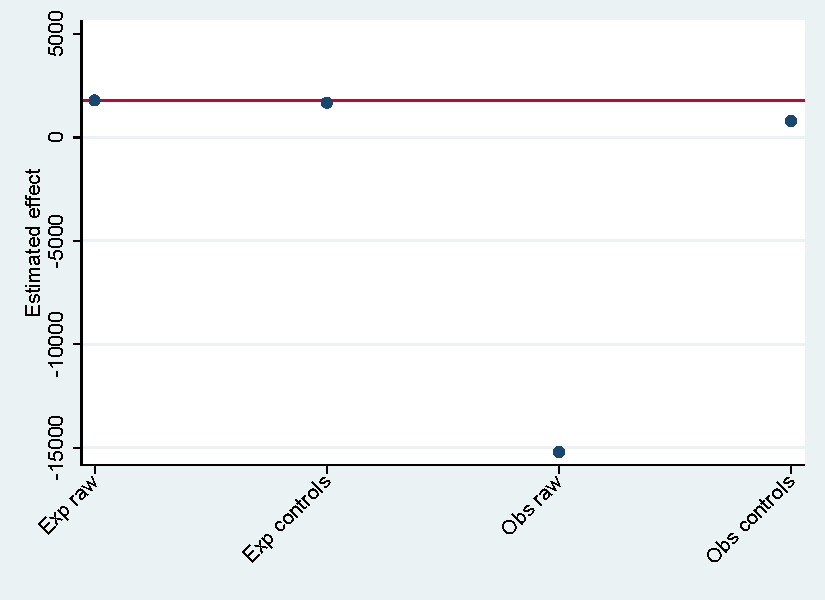
\includegraphics[width=\linewidth]{../output/estimates.pdf}

\end{document}
